% Architecture x mixer lattice — TikZ source. Compiles to a tight standalone
% PDF (pdflatex figures/architecture-lattice.tex), which `book-scaffold
% build-figures` converts to public/figures/architecture-lattice.svg.
%
% The composition chapter's two switches (bidirectional-vs-causal self-
% attention, cross-attention conditioning present-or-not) lifted to ANY
% sequence mixer: 3 patterns (rows) x 3 mixer families (columns) = 9
% coordinates. Eight carry a canonical named model; encoder-decoder x SSM
% (bottom-right) is structurally available but has no canonical instance —
% shown dashed. Pattern and mixer are orthogonal design axes throughout.
\documentclass[tikz,border=3pt]{standalone}
\usepackage{amsmath}
\usepackage{amssymb}
\usepackage{tikz}
\usetikzlibrary{positioning,arrows.meta,calc}
\begin{document}
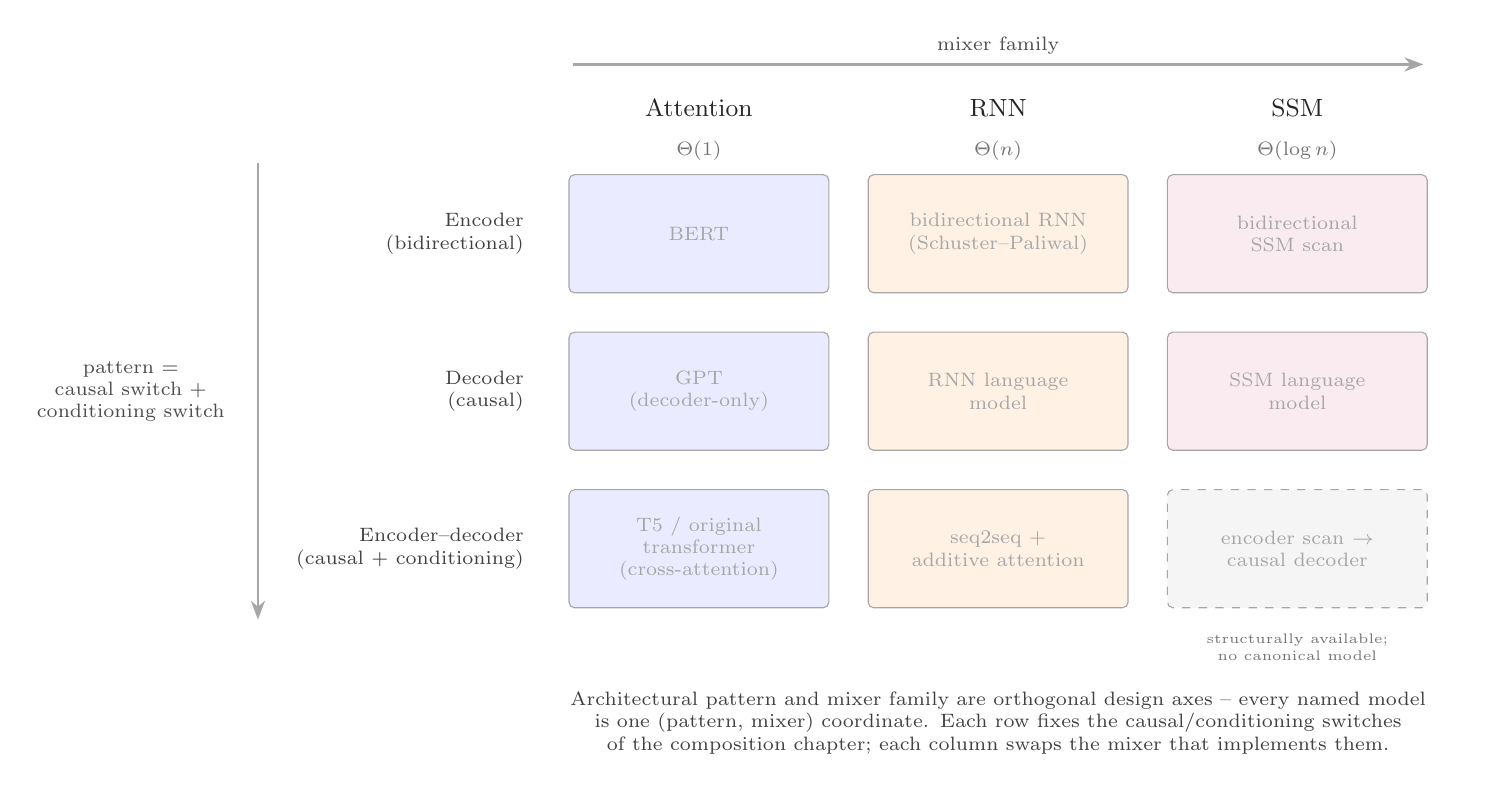
\begin{tikzpicture}[
    font=\small,
    box/.style={draw, gray!70, rounded corners=2pt, align=center,
                minimum height=15mm, minimum width=33mm, inner sep=3pt,
                font=\scriptsize},
    dbox/.style={box, dashed, fill=black!4},
    op/.style={->, >={Stealth[length=2.4mm]}, gray!70, thick},
    note/.style={font=\tiny, align=center, text=black!55},
  ]
  % --- grid geometry: columns = mixer family, rows = architectural pattern ---
  \def\colA{0}    \def\colB{3.8}  \def\colC{7.6}
  \def\rowA{0}    \def\rowB{-2.0} \def\rowC{-4.0}

  % --- top margin: horizontal axis arrow (mixer family) ---
  \draw[op] (-1.6,2.15) -- (9.2,2.15)
    node[midway, above, font=\scriptsize, text=black!70] {mixer family};

  % --- column headers + sequential-depth tags ---
  \node[font=\small, text=black!85] at (\colA,1.6) {Attention};
  \node[font=\small, text=black!85] at (\colB,1.6) {RNN};
  \node[font=\small, text=black!85] at (\colC,1.6) {SSM};
  \node[font=\scriptsize, text=black!55] at (\colA,1.05) {$\Theta(1)$};
  \node[font=\scriptsize, text=black!55] at (\colB,1.05) {$\Theta(n)$};
  \node[font=\scriptsize, text=black!55] at (\colC,1.05) {$\Theta(\log n)$};

  % --- row 1: Encoder (bidirectional) ---
  \node[box, fill=blue!8]    at (\colA,\rowA) {BERT};
  \node[box, fill=orange!10] at (\colB,\rowA)
    {bidirectional RNN\\(Schuster--Paliwal)};
  \node[box, fill=purple!8]  at (\colC,\rowA) {bidirectional\\SSM scan};

  % --- row 2: Decoder (causal) ---
  \node[box, fill=blue!8]    at (\colA,\rowB) {GPT\\(decoder-only)};
  \node[box, fill=orange!10] at (\colB,\rowB) {RNN language\\model};
  \node[box, fill=purple!8]  at (\colC,\rowB) {SSM language\\model};

  % --- row 3: Encoder-decoder (causal + conditioning) ---
  \node[box, fill=blue!8]    at (\colA,\rowC)
    {T5 / original\\transformer\\(cross-attention)};
  \node[box, fill=orange!10] at (\colB,\rowC)
    {seq2seq +\\additive attention};
  \node[dbox] (r3c3) at (\colC,\rowC) {encoder scan $\to$\\causal decoder};
  \node[note, below=2mm of r3c3] {structurally available;\\no canonical model};

  % --- row labels ---
  \node[font=\scriptsize, align=right, text=black!75, anchor=east]
    at (-2.1,\rowA) {Encoder\\(bidirectional)};
  \node[font=\scriptsize, align=right, text=black!75, anchor=east]
    at (-2.1,\rowB) {Decoder\\(causal)};
  \node[font=\scriptsize, align=right, text=black!75, anchor=east]
    at (-2.1,\rowC) {Encoder--decoder\\(causal + conditioning)};

  % --- left margin: vertical axis arrow (pattern = the two switches) ---
  \draw[op] (-5.6,0.9) -- (-5.6,-4.9);
  \node[font=\scriptsize, align=center, text=black!70, anchor=east]
    at (-5.9,\rowB) {pattern =\\causal switch +\\conditioning switch};

  \node[below, align=center, text width=11.5cm, font=\scriptsize, text=black!75]
    at (\colB,-5.7)
    {Architectural pattern and mixer family are orthogonal design axes --
     every named model is one (pattern, mixer) coordinate. Each row fixes the
     causal/conditioning switches of the composition chapter; each column
     swaps the mixer that implements them.};
\end{tikzpicture}
\end{document}
